\documentclass[11pt,letterpaper]{article}

\usepackage[margin=1in,headheight=14pt]{geometry}
\usepackage{amsmath,amssymb,amsthm,mathtools}
\usepackage{graphicx}
\usepackage{xcolor}
\usepackage{enumitem}
\usepackage{microtype}
\usepackage{fancyhdr}
\usepackage[colorlinks=true,linkcolor=blue,citecolor=blue,urlcolor=blue]{hyperref}

% Personal notation and theorem environments.
%!TEX root = EM_singular_models.tex

% PDF margin etc settings
%\setlength{\textwidth}{\paperwidth}
%\addtolength{\textwidth}{-6cm}
%\setlength{\textheight}{\paperheight}
%\addtolength{\textheight}{-4cm}
%\addtolength{\textheight}{-1.1\headheight}
%\addtolength{\textheight}{-\headsep}
%\addtolength{\textheight}{-\footskip}
%\setlength{\oddsidemargin}{0.5cm}
%\setlength{\evensidemargin}{0.5cm}

%%%%%%%%%%%%%%%%%%%%%%%%%%%%%%%%

% MACROS HERE

%%%%%%%%%%%%%%%%%%%%%%%%%%%%%%%%

\newcommand{\fixedpointtheta}{\widehat\theta_\obs}

\newcommand{\cover}{N}
\newcommand{\kinit}{\nu}
\newcommand{\cdelta}{c_\threshold}
\newcommand{\dndelta}{\omega}
\newcommand{\kndelta}{\Upsilon}
\newcommand{\kndeltanew}{\Psi}
\newcommand{\radii}{\mathcal{R}}
\newcommand{\event}{\mathcal{E}}
\newcommand{\kevent}{\mathcal{D}}


% Observations, dimension etc.
\newcommand{\dims}{\ensuremath{d}}
\newcommand{\samples}{\ensuremath{n}}
\newcommand{\obs}{\samples}
\newcommand{\real}{\ensuremath{\mathbb{R}}}
\newcommand{\complex}{\ensuremath{\mathbb{C}}}
\newcommand{\realdim}{\ensuremath{\real^\dims}}

\newcommand{\smallthreshold}{\epsilon}

% some mathcal notations
\newcommand{\order}[1]{\ensuremath{\mathcal{O}\parenth{#1}}}

% Basic statistics notation
\newcommand{\xstar}{\ensuremath{x^*}}
\newcommand{\xbar}{\ensuremath{\bar{x}}}
% True parameter
\newcommand{\thetastar}{\ensuremath{{\theta^*}}}
% Estimate one
\newcommand{\thetahat}{\ensuremath{\widehat{\theta}}}
% Estimate two
\newcommand{\thetatil}{\ensuremath{\widetilde{\theta}}}
\newcommand{\thetabar}{\ensuremath{\bar{\theta}}}
\newcommand{\yvec}{\ensuremath{y}}
\newcommand{\Xmat}{\ensuremath{X}}

% Distributions
\newcommand{\distribution}{P}
\newcommand{\density}{f}
\newcommand{\gaussiandensity}{\phi}
\newcommand{\NORMAL}{\ensuremath{\mathcal{N}}}
\newcommand{\BER}{\ensuremath{\mbox{Ber}}}

% Spaces
\newcommand{\Xspace}{\ensuremath{\mathcal{X}}}
\newcommand{\Yspace}{\ensuremath{\mathcal{Y}}}
\newcommand{\Zspace}{\ensuremath{\mathcal{Z}}}


% Brackets Size
\newcommand{\brackets}[1]{\left[ #1 \right]}
\newcommand{\parenth}[1]{\left( #1 \right)}
\newcommand{\bigparenth}[1]{\big( #1 \big)}
\newcommand{\biggparenth}[1]{\bigg( #1 \bigg)}
\newcommand{\braces}[1]{\left\{ #1 \right \}}
\newcommand{\abss}[1]{\left| #1 \right |}
\newcommand{\angles}[1]{\left\langle #1 \right \rangle}
\newcommand{\tp}{^\top}

% Generic vectors and scalars
\newcommand{\myvec}{u} % for generic vector
\newcommand{\myvectwo}{v} % for generic vector
\newcommand{\mymat}{B}
\newcommand{\set}{{A}}
\newcommand{\scalar}{\alpha}
\newcommand{\tvscalar}{\epsilon}
\newcommand{\tailboundscalar}{t}
\newcommand{\term}{U}
\newcommand{\myVarone}{\alpha_X}
\newcommand{\myVartwo}{\alpha_Y}
\newcommand{\myCovmat}{\Sigma}
\newcommand{\xcord}[1]{x^{(#1)}}
\newcommand{\xcordpop}[1]{X^{(#1)}}
\newcommand{\ycordpop}[1]{Y^{(#1)}}
\newcommand{\myVarthree}{\ensuremath{U}}
\newcommand{\myVarfour}{\ensuremath{V}}
\newcommand{\myfuntwo}{\ensuremath{g}}
\newcommand{\numsteps}{t}
\newcommand{\totalnumsteps}{T}
\newcommand{\seqalpha}[1]{\alpha_{#1}}
\newcommand{\seqnu}[1]{\nu^{(#1)}}
\newcommand{\imax}{\ell_\smallthreshold}
\newcommand{\basis}{e}
\newcommand{\radem}{\varepsilon}
\newcommand{\Tone}{T\ensuremath{_{0}}}
\newcommand{\Ttwo}{T\ensuremath{_{2}}}
\newcommand{\contractPar}[1]{\ensuremath{\gamma\parenth{#1}}}

\newcommand{\simiid}{\overset{\mathrm{i.i.d.}}{\sim}}
\newcommand{\eqd}{\overset{d}{=}}


% EM updates
\newcommand{\hidden}{Z}
\newcommand{\qfun}[2]{Q(#1\vert#2)}
\newcommand{\variable}{\theta}
\newcommand{\weights}{w}
\newcommand{\myfun}{q}
\newcommand{\gradf}{\nabla \myfun}
\newcommand{\hessf}{\nabla^2 \myfun}
\newcommand{\iter}{t}
\newcommand{\mupdate}{M}
\newcommand{\mupdategeneral}{\ensuremath{M^{GN}}}




% EM contractions
\newcommand{\contractgene}{\ensuremath{\gamma^{GN}}}
\newcommand{\updateMat}{\ensuremath{\Gamma_{\theta}}}
\newcommand{\mymatTheta}{\ensuremath{B_{\theta}}}
\newcommand{\sech}{\text{sech}}

% Nhat's macros 
\newcommand{\Rspace}{\ensuremath{\mathbb{R}}}
\newcommand{\Ecal}{\ensuremath{\mathcal{E}}}
\newcommand{\Ncal}{\ensuremath{\mathcal{N}}}
\newcommand{\gradient}{\ensuremath{\nabla}}
\newcommand{\smallweight}{\ensuremath{\epsilon^{sw}}}
\newcommand{\smallnorm}{\ensuremath{\rho^{sw}}}
\newcommand{\ball}{\ensuremath{\mathbb{B}}}
\newcommand{\sphere}{\ensuremath{\mathbb{S}}}

\newcommand{\diam}{\ensuremath{\text{diam}}}
\newcommand{\upper}{\ensuremath{\bar{C}}}
\newcommand{\sample}{\ensuremath{\xi}}
\newcommand{\weight}{\ensuremath{\pi}}
\newcommand{\contracasym}{\ensuremath{\rho}}
\newcommand{\Fishermatrix}{\ensuremath{\mathcal{I}}}
\newcommand{\barcontracasym}{\ensuremath{\bar{\rho}}}


\newcommand{\TrueDensity}{\ensuremath{f}}
\newcommand{\FitDensity}{\ensuremath{f}_{\theta}}
\newcommand{\FitDensityfree}{\ensuremath{f}_{\pi, \theta}}
\newcommand{\FitDensitygen}{\ensuremath{f}_{\pi, \theta_{1}, \theta_{2}}}
\newcommand{\FitDensitymore}{\ensuremath{f}_{G}}
\newcommand{\normden}{\ensuremath{\phi}}
\newcommand{\mean}{\ensuremath{\theta}}
\newcommand{\sd}{\ensuremath{\sigma}}
\newcommand{\parFOS}{\ensuremath{\gamma}}
\newcommand{\funQ}{\ensuremath{Q}}
\newcommand{\updateM}{\ensuremath{M}}
\newcommand{\weightFun}{\ensuremath{w}}
\newcommand{\mydefn}{\ensuremath{:=}}
\newcommand{\poincare}{\ensuremath{\tilde{C}}}
\newcommand{\paraspace}{\ensuremath{\Theta}}
\newcommand{\loglihood}{\ensuremath{F}}
\newcommand{\prior}{\ensuremath{\pi}}
\newcommand{\posterior}{\ensuremath{\Pi}}
\newcommand{\boundcons}{\ensuremath{B}}
\newcommand{\boundconstot}{\ensuremath{H}}
\newcommand{\noise}{\ensuremath{\varepsilon}}
\newcommand{\loglihoodgaus}{\ensuremath{F^{G}}}
\newcommand{\loglihoodind}{\ensuremath{F^{I}}}
\newcommand{\loglihoodlogit}{\ensuremath{F^{R}}}
\newcommand{\noiseone}{\ensuremath{\varepsilon_{1}}}
\newcommand{\noisetwo}{\ensuremath{\varepsilon_{2}}}

%%%SDE_Bayesian_inf
\newcommand{\weakcon}{\ensuremath{\psi}}
\newcommand{\perturb}{\ensuremath{\zeta}}
\newcommand{\inver}{\ensuremath{\xi}}

% Universal constants
\newcommand{\unicon}{c}
\newcommand{\uniconnew}{c'}
\newcommand{\uniconone}{c_1}
\newcommand{\unicontwo}{c_2}

% some parameters that you may define
\newcommand{\scparam}{m} % strong  convexity parameter
\newcommand{\smoothness}{L} % smoothness parameter
\newcommand{\step}{h}


%%%%%%%%% Distributions and Random variables %%%%%%%%%%%
\newcommand{\rvg}{\xi} % to denote the random variable g
\newcommand{\threshold}{\delta}


%%%%%%%%% Basic Terms like defn, etal, tmix, polylog %%%%%%%%%%%
\newcommand{\defn}{:=}
\newcommand{\rdefn}{=:}
\newcommand{\etal}{{et al.}}
\newcommand{\polylog}{\text{poly-log}}

% Some vector/matrix norms
\newcommand{\matnorm}[3]{|\!|\!| #1 | \! | \!|_{{#2}, {#3}}}
\newcommand{\matsnorm}[2]{|\!|\!| #1 | \! | \!|_{{#2}}}
\newcommand{\vecnorm}[2]{\left\| #1\right\|_{#2}}
\newcommand{\enorm}[1]{\vecnorm{#1}{2}} % euclidean norm
\newcommand{\nucnorm}[1]{\ensuremath{\matsnorm{#1}{\footnotesize{\mbox{nuc}}}}}
\newcommand{\fronorm}[1]{\ensuremath{\matsnorm{#1}{\footnotesize{\mbox{fro}}}}}
\newcommand{\opnorm}[1]{\ensuremath{\matsnorm{#1}{\tiny{\mbox{op}}}}}
%%% EM paper
\newcommand{\constrainnorm}[1]{\vecnorm{#1}{[k]}} % euclidean norm

\newcommand{\bigmatsnorm}[2]{{\Big|\!\Big|\!\Big| #1
  \Big|\!\Big|\!\Big|}_{#2}}

% Inner product
\newcommand{\inprod}[2]{\ensuremath{\langle #1 , \, #2 \rangle}}

% Kullback-Leibler
\newcommand{\kull}[2]{\ensuremath{D_{\text{KL}}(#1\; \| \; #2)}}

% Probability
\newcommand{\Exs}{\ensuremath{{\mathbb{E}}}}
\newcommand{\Prob}{\ensuremath{{\mathbb{P}}}}

%Eigenvector / eigenvalue related notation
\newcommand{\eig}[1]{\ensuremath{\lambda_{#1}}}
\newcommand{\eigmax}{\ensuremath{\eig{\max}}}
\newcommand{\eigmin}{\ensuremath{\eig{\min}}}

% \DeclareMathOperator{\det}{det}
\DeclareMathOperator{\modd}{mod}
\DeclareMathOperator{\diag}{diag}
\DeclareMathOperator{\var}{var}
\DeclareMathOperator{\cov}{cov}
\DeclareMathOperator{\trace}{trace}
\DeclareMathOperator{\abs}{abs}
\DeclareMathOperator{\floor}{floor}
\DeclareMathOperator{\vol}{vol}
\DeclareMathOperator{\child}{child}
\DeclareMathOperator{\parent}{parent}
\DeclareMathOperator{\sign}{sign}
\DeclareMathOperator{\rank}{rank}
\DeclareMathOperator{\toeplitz}{toeplitz}




\newtheoremstyle{named}{}{}{\itshape}{}{\bfseries}{.}{.5em}{\thmnote{#3's }#1}
\theoremstyle{named}
\newtheorem*{namedtheorem}{Lemma}

%%%%%%%
\theoremstyle{plain}

% {Theorem, Proposition, Lemma, Corollary} numbered sequentially
% throughout the paper
\newtheorem{theorem}{Theorem}
\newtheorem{proposition}{Proposition}
\newtheorem{lemma}{Lemma}
\newtheorem{claim}{Claim}
\newtheorem{corollary}{Corollary}
\newtheorem{definition}{Definition}
\newtheorem{conjecture}{Conjecture}
\newtheorem{remark}{Remark}
%%%%%%%%%%%%%%%%%%%%%%%%%%%%%%%%%%%%%%%%%%%%%%%%%%%%%%%%%%%%%%%%%%%%%%%
% WIDEBAR COMMAND
\newlength{\widebarargwidth}
\newlength{\widebarargheight}
\newlength{\widebarargdepth}
\DeclareRobustCommand{\widebar}[1]{%
  \settowidth{\widebarargwidth}{\ensuremath{#1}}%
  \settoheight{\widebarargheight}{\ensuremath{#1}}%
  \settodepth{\widebarargdepth}{\ensuremath{#1}}%
  \addtolength{\widebarargwidth}{-0.3\widebarargheight}%
  \addtolength{\widebarargwidth}{-0.3\widebarargdepth}%
  \makebox[0pt][l]{\hspace{0.3\widebarargheight}%
    \hspace{0.3\widebarargdepth}%
    \addtolength{\widebarargheight}{0.3ex}%
    \rule[\widebarargheight]{0.95\widebarargwidth}{0.1ex}}%
  {#1}}



%%% New version of \caption puts things in smaller type, single-spaced
%%% and indents them to set them off more from the text.
\makeatletter
\long\def\@makecaption#1#2{
        \vskip 0.8ex
        \setbox\@tempboxa\hbox{\small {\bf #1:} #2}
        \parindent 1.5em  %% How can we use the global value of this???
        \dimen0=\hsize
        \advance\dimen0 by -3em
        \ifdim \wd\@tempboxa >\dimen0
                \hbox to \hsize{
                        \parindent 0em
                        \hfil
                        \parbox{\dimen0}{\def\baselinestretch{0.96}\small
                                {\bf #1.} #2
                                %%\unhbox\@tempboxa
                                }
                        \hfil}
        \else \hbox to \hsize{\hfil \box\@tempboxa \hfil}
        \fi
        }
\makeatother



%% COMMENTING commands

\long\def\comment#1{}
\definecolor{battleshipgrey}{rgb}{0.52, 0.52, 0.51}
\definecolor{darkgray}{rgb}{0.66, 0.66, 0.66}
\definecolor{darkgreen}{rgb}{0.0, 0.2, 0.13}
\definecolor{darkspringgreen}{rgb}{0.09, 0.45, 0.27}
\definecolor{dukeblue}{rgb}{0.0, 0.0, 0.61}
\definecolor{olivedrab7}{rgb}{0.24, 0.2, 0.12}
\definecolor{darkblue}{rgb}{0.0, 0.0, 0.55}
\definecolor{darkscarlet}{rgb}{0.34, 0.01, 0.1}
\definecolor{candyapplered}{rgb}{1.0, 0.03, 0.0}
\definecolor{ao(english)}{rgb}{0.0, 0.5, 0.0}
\definecolor{applegreen}{rgb}{0.55, 0.71, 0.0}

\newcommand{\red}[1]{\textcolor{red}{#1}}
\newcommand{\mjwcomment}[1]{{\bf{{\red{{MJW --- #1}}}}}}
\newcommand{\mwlcomment}[1]{{\bf{{\color{orange}{{Wenlong --- #1}}}}}}

\newcommand{\blue}[1]{\textcolor{blue}{#1}}
\newcommand{\green}[1]{\textcolor{green}{#1}}
\newcommand{\highlight}[1]{\textcolor{applegreen}{#1}}

% comment lines
\newcommand{\genecomment}[1]{{\bf{{\blue{{TEAM --- #1}}}}}}
\newcommand{\rrdcomment}[1]{{\bf{{\blue{{RRD --- #1}}}}}}
\newcommand{\nhcomment}[1]{{\bf{{\blue{{NH --- #1}}}}}}
\newcommand{\kkcomment}[1]{{\bf{{\darkgreen{{KK --- #1}}}}}}


\newcommand{\widgraph}[2]{\includegraphics[keepaspectratio,width=#1]{#2}}


\newcommand{\coursenumber}{STA3000F}
\newcommand{\coursetitle}{Advanced Theory of Statistics}
\newcommand{\courseterm}{Fall 2026}
\newcommand{\lecturenumber}{1}
\newcommand{\lecturedate}{September 11, 2026}
\newcommand{\lecturer}{Wenlong Mou}

\pagestyle{fancy}
\fancyhf{}
\fancyhead[L]{\coursenumber: \coursetitle}
\fancyhead[R]{Lecture \lecturenumber}
\fancyfoot[C]{\lecturenumber--\arabic{page}}
\renewcommand{\headrulewidth}{0.4pt}
\renewcommand{\footrulewidth}{0pt}

\usepackage{bm}

\setcounter{section}{\numexpr\lecturenumber-1\relax}
\renewcommand{\thepage}{\lecturenumber--\arabic{page}}

\newtheorem{example}{Example}

\newcommand{\makelecturenotesheader}{%
  \noindent
  \textbf{\coursenumber: \coursetitle}%
  \hfill
  \textbf{\courseterm}

  \begin{center}
    {\Large\bfseries Lecture \lecturenumber: \lecturedate}
  \end{center}

  \noindent
  \textbf{Lecturer:} \lecturer
  \par\medskip
  \hrule
  \bigskip
}

\begin{document}

\makelecturenotesheader

\section{Logistics}
\begin{itemize}
  \item Course website: \url{mouwenlong.github.io/teaching/sta3000f26}
  \item Grading: take-home exam + project
\end{itemize}

\subsection{Outline}
\begin{itemize}
\item Basic probability theory review (concentration inequalities)
\item Decision theory (minimax, Bayes, admissibility)
\item Modern tools (empirical processes)
\item Basics of nonparametric statistics (density estimation, regression)
\end{itemize}

\section{Probability review}
\subsection{Radon--Nikodym derivative}
Idea: generalize probability density function to general measures.
\begin{itemize}
  \item $\mu$ measure of interest
  \item $\nu$ reference measure
\end{itemize}
We say $\mu$ is \emph{absolutely continuous} with respect to $\nu$ if $\nu(A) = 0 \implies \mu(A) = 0$. In this case, there exists a function $f$ such that
\begin{align*}
  f (x) = \frac{d\mu}{d\nu}(x) \quad \text{for $\nu$-almost every $x$}.
\end{align*}
For any measurable set $A$, we have
\begin{align*}
  \mu (A) = \int_A f(x) d\nu(x).
\end{align*}
\subsection{Basic probability inequalities}
\paragraph{Markov inequality}
For a non-negative random variable $X$ and any $a > 0$,
\begin{align*}
  \mathbb{P}(X \geq a) \leq \frac{\mathbb{E}[X]}{a}.
\end{align*}
Proof: 
\begin{align*}
  \Prob (X \geq a) = \Exs \big[ \bm{1}_{X \geq a} \big] \leq \Exs \big[ \frac{X}{a} \bm{1}_{X \geq a} \big] \leq \frac{\Exs [X]}{a}.
\end{align*}
Remark: as $a \rightarrow \infty$, the tail probability $\Prob (X \geq a)$ decays at least as fast as $1/a$. This is a very weak bound.

\paragraph{Chebyshev inequality:}
For a random variable $X$ with finite mean $\mu$ and finite non-zero variance $\sigma^2$, and any $a > 0$,
\begin{align*}
  \mathbb{P}(|X - \mu| \geq a) \leq \frac{\sigma^2}{a^2}.
\end{align*}
Proof: by Markov inequality, we have
\begin{align*}
  \Prob (|X - \mu| \geq a) = \Exs \big[ \bm{1}_{|X - \mu| \geq a} \big] \leq \Exs \big[ \frac{(X - \mu)^2}{a^2} \bm{1}_{|X - \mu| \geq a} \big] \leq \frac{\Exs [(X - \mu)^2]}{a^2} = \frac{\sigma^2}{a^2}.
\end{align*}
Remark: second moment gives a better bound than the first moment. As $a \rightarrow \infty$, the tail probability $\Prob (|X - \mu| \geq a)$ decays at least as fast as $1/a^2$.

\paragraph{Higher moments?} Suppose that the random variable $X$ has finite $k$-th moment $\Exs[|X|^k] < \infty$ for some $k > 0$. Then, for any $a > 0$,
\begin{align*}
  \Prob (|X - \Exs [X] | \geq a) \leq \frac{\Exs [|X - \Exs [X]|^k]}{a^k}.
\end{align*}
Can we get a faster decay? Exponential decay?

\paragraph{Moment generating function (MGF):} For a random variable $X$, the moment generating function is defined as
\begin{align*}
  m_X(t) = \Exs [e^{tX}], \quad t \in \mathbb{R}.
\end{align*}
Why is it called ``moment generating function''? Taylor expansion of $m_X(t)$ at $t = 0$ gives
\begin{align*}
  m_X(t) = \Exs [e^{tX}] = \sum_{k=0}^{\infty} \frac{t^k}{k!} \Exs [X^k].
\end{align*}
So if you take higher order derivatives of $m_X(t)$ at $t = 0$, you can get the moments of $X$.
\begin{itemize}
  \item $X \sim \mathcal{N} (\mu, \sigma^2)$, then $m_X(t) = e^{\mu t + \frac{1}{2} \sigma^2 t^2}$.
  \item $X \sim \text{Bernoulli}(p)$, then $m_X(t) = 1 - p + p e^t$.
\end{itemize}
Note: moment generating function may not exist for all $t \in \mathbb{R}$, e.g., Cauchy distribution (moment does not even exist); exponential distribution (moment generating function only exists for $t < \lambda$).

\bigskip

By applying Markov inequality to $e^{t (X - \Exs [X])}$, we have
\begin{align*}
  \Prob (X - \Exs [X] \geq a) = \Prob (e^{t (X - \Exs [X])} \geq e^{ta}) \leq \frac{\Exs [e^{t (X - \Exs [X])}]}{e^{ta}} = e^{-ta} m_X(t) e^{-t\Exs [X]}.
\end{align*}
Note: this holds for any $t > 0$. So we can take infimum over $t > 0$ to get the best bound.

\begin{example}
  For $X \sim \mathcal{N} (\mu, \sigma^2)$, we have
  \begin{align*}
    \Prob (X \geq \mu + a) \leq e^{- ta} m_X(t) e^{-t\mu} = e^{-ta} e^{\mu t + \frac{1}{2} \sigma^2 t^2} e^{-t\mu} = e^{-ta + \frac{1}{2} \sigma^2 t^2}.
  \end{align*}
  Take the optimal choice of $t = a / \sigma^2$, we have
  \begin{align*}
    \Prob (X \geq \mu + a) \leq e^{- \frac{a^2}{2\sigma^2}}.
  \end{align*}
\end{example}
For normal distribution, we know the exact tail probability. But for more general distributions, we can use moment generating function to get a bound on the tail probability.

\begin{definition}
  $X$ is called \emph{sub-Gaussian} if there exists a constant $\sigma > 0$ such that for all $t \in \mathbb{R}$,
  \begin{align*}
    \Exs [e^{t (X - \Exs [X])}] \leq e^{\frac{1}{2} \sigma^2 t^2}.
  \end{align*} 
\end{definition}
e.g. Rademacher random variable $X$ with $\Prob (X = 1) = \Prob (X = -1) = 1/2$.
\begin{align*}
  m_X(t) = \Exs [e^{tX}] &= \frac{1}{2} e^t + \frac{1}{2} e^{-t} = \cosh (t)\\
  &\leq 1 + \frac{t^2}{2} + \frac{t^4}{4!} + \frac{t^6}{6!} + \cdots
\end{align*}
On the other hand, we have
\begin{align*}
  e^{\frac{1}{2} t^2} = 1 + \frac{t^2}{2} + \frac{t^4}{2^2 2!} + \frac{t^6}{2^3 3!} + \cdots
\end{align*}
Term-wise comparison shows that $\cosh (t) \leq e^{\frac{1}{2} t^2}$ for all $t \in \mathbb{R}$. So Rademacher random variable is sub-Gaussian with $\sigma = 1$.

\bigskip

\paragraph{Sum (average) of $\mathrm{i.i.d.}$ random variables:} Let $X_1, \ldots, X_n$ be $\mathrm{i.i.d.}$ sub-Gaussian random variables with parameter $\sigma$. Can we say something about $\frac{1}{n} \sum_{i=1}^n X_i$?

For any $t \in \mathbb{R}$, we have
\begin{align*}
  \Exs \Big[ e^{t \left( \frac{1}{n} \sum_{i=1}^n X_i - \Exs [X_i] \right)} \Big] = \Big\{ \Exs \Big[ e^{\frac{t}{n} (X_1 - \Exs [X_1])} \Big] \Big\}^n = \Big\{ m_{X_1}(t/n) \Big\}^n \leq \exp \Big(  \frac{ \sigma^2 t^2}{2n} \Big).
\end{align*}
So, the average is $\frac{\sigma}{\sqrt{n}}$-sub-Gaussian, and consequently,
\begin{align*}
  \Prob \Big( \frac{1}{n} \sum_{i=1}^n X_i - \Exs [X_i] \geq a \Big) \leq e^{-ta} m_{X_1 - \Exs [X_1]}(t/n)^n \leq e^{-ta + \frac{\sigma^2 t^2}{2n}}.
\end{align*}
Taking the optimal choice of $t = an / \sigma^2$, we have
\begin{align*}
  \Prob \Big( \frac{1}{n} \sum_{i=1}^n X_i - \Exs [X_i] \geq a \Big) \leq e^{- \frac{n a^2}{2\sigma^2}}.
\end{align*}
This is called Hoeffding's inequality. It shows that the average of $\mathrm{i.i.d.}$ sub-Gaussian random variables concentrates around its mean with exponential decay.

e.g. $X_1, \cdots, X_n$ are $\mathrm{i.i.d.}$ Rademacher random variables. Then, for any $a > 0$,
\begin{align*}
  \Prob \Big( \big| \frac{1}{n} \sum_{i = 1}^n X_i \big| \geq a \Big) \leq 2 e^{- \frac{n a^2}{2}},
\end{align*}
where the factor of $2$ comes from the union bound.

\bigskip

In general, we can also use the same idea to study $\mathrm{i.i.d.}$ average of bounded random variables. Let $X_1, \ldots, X_n$ be $\mathrm{i.i.d.}$ random variables with $\Exs [X_i] = \mu$ and $X_i \in [a, b]$ almost surely. We can show that $X_i - \mu$ is sub-Gaussian with parameter $\sigma = \frac{b - a}{2}$. Then, we have
\begin{align*}
  \Prob \Big( \big| \frac{1}{n} \sum_{i = 1}^n X_i - \mu \big| \geq u \Big) \leq 2\exp \Big( - \frac{2 n u^2}{(b - a)^2} \Big). 
\end{align*}
Remarks:
\begin{itemize}
  \item Deviation is of order $O(1/\sqrt{n})$. Tail decay is exponential.
  \item Independence is needed in general (can be extended when specific dependence structure is known. e.g. martingale difference sequence). Identical distribution can be relaxed in most cases, as long as we have the MGF bound for each random variable.
\end{itemize}

\paragraph{Union bound}
\begin{align*}
  \Prob \Big( \bigcup_{i \in \mathcal{I}} A_i \Big) \leq \sum_{i \in \mathcal{I}} \Prob(A_i).
\end{align*}
Remark:
\begin{itemize}
  \item Usually, each $A_i$ corresponds to ``bad event at certain direction''. If none of them is happening, then we are in a ``good event''.
  \item In many cases, we have exponentially many bad events. That's why we need the tail probability to decay exponentially fast, so that the union bound still gives a meaningful bound.
\end{itemize}

\paragraph{Example: probabilistic method in combinatorics.} Consider Hamming cube $\{-1 , + 1\}^n$. Hamming distance between two points $x, y \in \{-1, +1\}^n$ is defined as
\begin{align*}
  d_H(x, y) = \sum_{i=1}^n \bm{1}_{x_i \neq y_i}.
\end{align*}
Question: can we pack a lot of points in the Hamming cube such that any two points are far away from each other? Concretely, we want to find a subset $S \subset \{-1, +1\}^n$ such that for any $x, y \in S$, $d_H(x, y) \geq n/4$.

Answer: $S$ can be exponentially large in $n$.

Let $X_1, X_2, \cdots, X_M \simiid \mathrm{Unif} \big( \{-1, 1\}^n \big)$. For each fixed $i, j$ pair, we have
\begin{align*}
 \Prob \big( d_H(X_i, X_j) < n/4 \big) = \Prob \Big( \sum_{k=1}^n \bm{1}_{X_{ik} \neq X_{jk}} < n/4 \Big) \leq \exp \Big( - 2n (1/4)^2 \Big) = e^{-n/8},
\end{align*}
where we used Hoeffding's inequality for sum of $\mathrm{i.i.d.}$ Bernoulli random variables.

Applying union bound, we have
\begin{align*}
  \Prob \Big( \exists i < j \text{ such that } d_H(X_i, X_j) < n/4 \Big) \leq \binom{M}{2} e^{-n/8} \leq \frac{M^2}{2} e^{-n/8}.
\end{align*}
We just need a ``good'' configuration to exist. So we want the probability of the bad event to be strictly less than $1$. By choosing $M = \lfloor e^{n/16} \rfloor$, we have
\begin{align*}
  \Prob \Big( \exists i < j \text{ such that } d_H(X_i, X_j) < n/4 \Big) \leq \frac{1}{2}.
\end{align*}

\section{Back to statistics -- decision theory}
Key question: how to compare different statistical procedures? And how to rigorously define ``optimal'' procedure? This requires a unified framework.


To start with, we define
\begin{itemize}
  \item A statistical model $\mathcal{P} = \{ P_\theta : \theta \in \Theta \}$, where $\Theta$ is the parameter space (here the ``parameter'' does not have to be finite-dimensional).
  \item Observe $X \sim P_{\theta^*}$ for some unknown $\theta^* \in \Theta$. Goal: to make decision about $\theta^*$ based on $X$.
  \item Decision rule $\delta: \mathcal{X} \rightarrow \mathcal{A}$, where $\mathcal{A}$ is the action space. For example, if we want to estimate $\theta^*$, then $\mathcal{A} = \Theta$; for testing hypothesis, $\mathcal{A} = \{0, 1\}$.
  \item Loss function $L: \Theta \times \mathcal{A} \rightarrow \mathbb{R}_+$, e.g., $L(\theta, a) = \|\theta - a\|^2$ for squared error loss; 0-1 loss for testing hypothesis.
  \item Risk function: expected loss of a decision rule $\delta$ when data is generated from $P_\theta$:
  \begin{align*}
    R (\theta; \delta) \mydefn \Exs_{X \sim P_\theta} [L(\theta, \delta(X))].
  \end{align*}
\end{itemize}
e.g. for estimation, consider a known functional $g : \Theta \rightarrow \mathbb{R}^d$. A decision rule $\delta$ is an estimator of $g(\theta^*)$. The risk function is
\begin{align*}
  R (\theta; \delta) = \Exs_{X \sim P_\theta} [\|\delta(X) - g(\theta)\|^2].
\end{align*}
e.g. for testing, we partition the parameter space into two disjoint sets $\Theta_0$ and $\Theta_1$. The null hypothesis is $H_0: \theta^* \in \Theta_0$ and the alternative hypothesis is $H_1: \theta^* \in \Theta_1$. A decision rule $\delta$ is a test of the hypothesis, where $\delta(X) = 0$ means we accept $H_0$ and $\delta(X) = 1$ means we reject $H_0$. The risk function is
\begin{align*}
  R (\theta; \delta) = \Exs_{X \sim P_\theta} [\bm{1}_{\{\delta(X) \neq \bm{1}_{\{\theta \in \Theta_1\}}\}}] = 
  \begin{cases}
    \Prob_{X \sim P_\theta} (\text{reject } H_0), & \text{if } \theta \in \Theta_0,\\
    \Prob_{X \sim P_\theta} (\text{accept } H_0), & \text{if } \theta \in \Theta_1.
  \end{cases}
\end{align*}

\begin{itemize}
  \item Smaller risk is better.
  \item Risk is a function of $\theta$. This becomes a multi-objective optimization problem.
  \item We may not be able to find a decision rule that is uniformly better than all other decision rules. So we need to define some optimality criteria.
\end{itemize}

\subsection{Admissibility}
\begin{definition}
  Let $\delta$ be a decision rule. We say $\delta$ is \emph{inadmissible} if there exists another decision rule $\widetilde{\delta}$ such that
  \begin{align*}
    R(\theta; \widetilde{\delta}) \leq R(\theta; \delta) \quad \text{for all } \theta \in \Theta,
  \end{align*}
  and the inequality is strict for at least one $\theta \in \Theta$. Otherwise, we say $\delta$ is \emph{admissible}.
\end{definition}

\paragraph{Problem 1:} stupid estimators can also be admissible.

e.g. $X_1, X_2, \cdots, X_n \simiid \mathcal{N} (\theta, 1)$, $\theta \in \mathbb{R}$. Consider $\thetahat (X) = 0$. Always output $0$ regardless of the data. Then, the risk function is
\begin{align*}
  R (\theta; \thetahat) = \Exs_{X \sim P_\theta} [(\thetahat(X) - \theta)^2] = \theta^2.
\end{align*}
The risk of this estimator at $0$ is $0$. So any other estimator ${\thetahat}'$ that dominates $\thetahat$ must have $R(0; {\thetahat}') = 0$. This means that ${\thetahat}'(X) = 0$ almost surely when $\theta = 0$. So ${\thetahat}'$ cannot dominate $\thetahat$. Therefore, $\thetahat$ is admissible.

\paragraph{Problem 2:} ``good'' estimators can be inadmissible.

``Stein's paradox'': $X_1, X_2, \cdots, X_n \simiid \mathcal{N} (\theta, I_d)$, $\theta \in \mathbb{R}^d$. Consider a simple estimator
\begin{align*}
  \thetahat_n \mydefn \frac{1}{n} \sum_{i=1}^n X_i.
\end{align*}
\begin{theorem}[Stein's paradox]
  If $d \geq 3$, then $\thetahat_n$ is inadmissible under squared error loss.
\end{theorem}
Proof: by construction. James--Stein estimator:
\begin{align*}
  \thetahat_{\mathrm{JS}} = \Big(1 - \frac{(d - 2)}{ n \vecnorm{\widebar{X}_n}{2}^2} \Big) \widebar{X}_n.
\end{align*}
We can calculate
\begin{align*}
  \Exs_\theta \big[ \vecnorm{\thetahat_{\mathrm{JS}} - \theta}{2}^2 \big] = \frac{d}{n} - \Exs \Big[ \Big( \frac{(d - 2)}{ n \vecnorm{\widebar{X}_n}{2}^2} \Big)^2 \Big] < \frac{d}{n} = \Exs_\theta \big[ \vecnorm{\bar{X}_n - \theta}{2}^2 \big]. 
\end{align*}
This proves the inadmissibility of $\widebar{X}_n$.

\bigskip
Remarks:
\begin{itemize}
  \item Sample mean is still ``good'' in many senses, e.g., it is minimax optimal. Even being inadmissible, the gap between sample mean and JS estimator is diminishing fast when $\vecnorm{\theta}{2}$ becomes large. In practice, it's not always making a big difference.
  \item JS estimator itself is also inadimissible, e.g. clip the factor when it goes below 0.
  \item JS estimator itself is useful. It shrinks towards 0 adaptively based on the data you see. So shrinkage improves the risk at $0$ without hurting the risk at non-zero. Related to modern topics including empirical Bayes estimation.
\end{itemize}
\begin{center}
  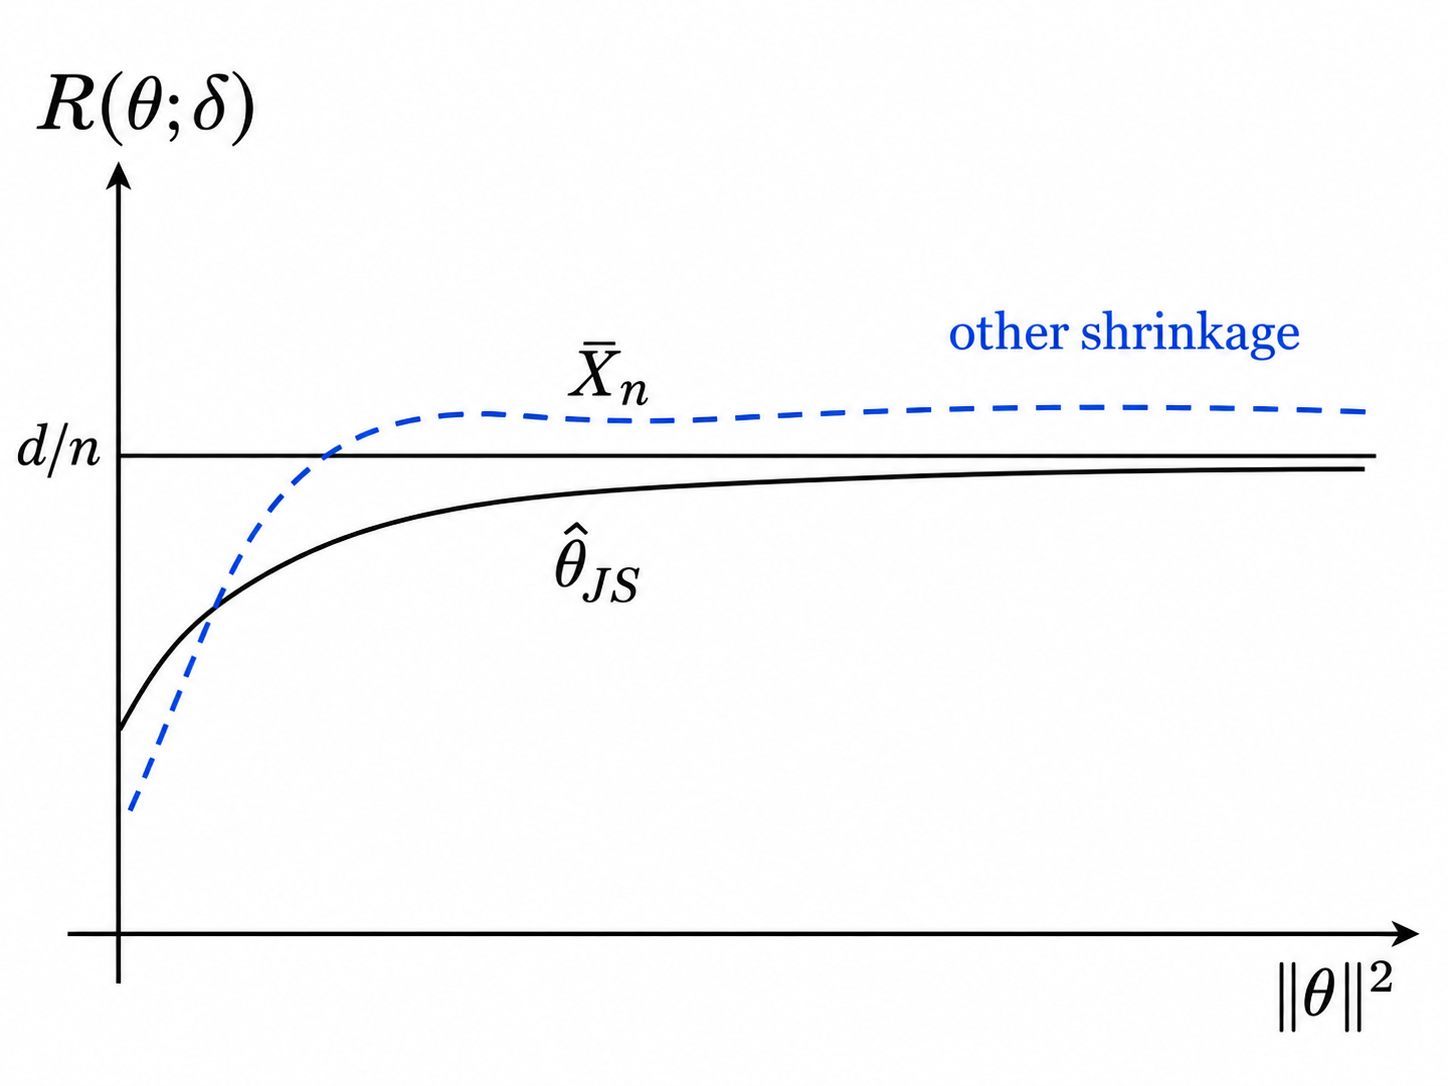
\includegraphics[width=0.5\textwidth]{./lec1-js-illustration.png}
\end{center}

\subsection{Bayes criterion}
Warning: most of this class is based on a frequentist perspective. But we will also discuss some Bayesian ideas. Here, the prior should be interpreted more as a weighting function on the parameter space, rather than a subjective belief about the parameter.

\begin{definition}
  Given a prior distribution $\pi$ on $\Theta$, the Bayes risk of a decision rule $\delta$ is defined as
  \begin{align*}
    r_\pi (\delta) \mydefn \int_\Theta R (\theta; \delta) d\pi(\theta) = \Exs_{\theta \sim \pi} [R (\theta; \delta)].
  \end{align*}
\end{definition}
This becomes a single-objective optimization problem. A decision rule $\delta_\pi$ is called a Bayes rule with respect to prior $\pi$ if it minimizes the Bayes risk:
\begin{align*}
  r_\pi (\delta_\pi) = \inf_{\delta} r_\pi (\delta).
\end{align*}

\paragraph{How to find the Bayes rule?} Suppose that $p_\theta (x) = \frac{d \Prob_\theta}{ d \lambda} (x)$ is the density of $P_\theta$ with respect to a reference measure $\lambda$. Then, we have
\begin{align*}
  r_\pi (\delta) &= \int_\Theta \int_\mathcal{X} L(\theta, \delta(x)) p_\theta (x) d\lambda(x) d\pi(\theta)\\
  &\stackrel{\mathrm{(Fubini-Tonelli)}}{=} \int_\mathcal{X} \underbrace{\int_\Theta L(\theta, \delta(x)) p_\theta (x) d\pi(\theta)}_{\textbf{We can pointwise minimize this for each $x$}} d\lambda(x).
\end{align*}
For each $x \in \mathcal{X}$, we can find $\delta_\pi(x)$ that minimizes the inner integral, i.e.,
\begin{align}
  \delta_\pi(x) = \arg\min_{a \in \mathcal{A}} \int_\Theta L(\theta, a) p_\theta (x) d\pi(\theta).\label{eq:bayes-rule-ptwise-minimization}
\end{align}
In Bayesian statistics, we see $\theta \sim \pi$ as a random variable. Then, the posterior distribution of $\theta$ given $X = x$ is
\begin{align*}
 d \Pi (\theta \mid X) = \frac{p_\theta (x) d\pi(\theta)}{\int_\Theta p_{\theta'} (x) d\pi(\theta')}.
\end{align*}
Consider the posterior expected loss:
\begin{align*}
  \Exs_{\theta \sim \Pi(\cdot \mid X)} [L(\theta, a)] = \int_\Theta L(\theta, a) d\Pi (\theta \mid X) = \frac{\int_\Theta L(\theta, a) p_\theta (x) d\pi(\theta)}{\int_\Theta p_{\theta'} (x) d\pi(\theta')}.
\end{align*}
Operationally, this is the conditional expected loss by choosing $a$ after observing $X = x$.

The denominator does not depend on $a$. So minimizing the posterior expected loss is equivalent to minimizing the numerator, which is exactly the same as \eqref{eq:bayes-rule-ptwise-minimization}. So, Bayes rule is equivalent to minimizing the posterior expected loss for each $X$.
\begin{align*}
  \delta_\pi(X) = \arg\min_{a \in \mathcal{A}} \Exs_{\theta \sim \Pi(\cdot \mid X)} [L(\theta, a)].
\end{align*}
For estimation problem with squared loss, i.e., $L(\theta, a) = \vecnorm{a - g(\theta)}{2}^2$, we have
\begin{align*}
  \delta_\pi(X) = \arg\min_{a \in \real^k} \int_\Theta \vecnorm{a - g (\theta)}{2}^2 d\Pi (\theta \mid X) = \int g (\theta) d \Pi (\theta \mid X).
\end{align*}
So the Bayes estimator is the posterior mean of $g(\theta)$. In practice, we usually use MCMC or variational inference to approximate the posterior distribution and compute the posterior mean.

\end{document}
